\documentclass{article}

\usepackage[margin=1in]{geometry}
\usepackage{graphicx}
\usepackage{subcaption}
\usepackage{times}
\usepackage{natbib}

\graphicspath{{figures/}} % DO NOT REMOVE OR FIGURES WILL NOT BE FOUND

\title{Symbolic Reasoning Gone Awry: Unexpected Pitfalls in Deep Model Clustering}
\author{
    Anonymous Submission
}
\date{}

\begin{document}

\maketitle

\begin{abstract}
Deep clustering methods have increasingly been used to tackle symbolic or compositional tasks, yet they often exhibit surprising drawbacks when exposed to complexities such as varying K-values or incomplete supervision. In a real-world deployment context, these pitfalls can lead to unreliable or misleading results. We investigate these vulnerabilities through controlled experiments and highlight lessons that can help practitioners avoid similar pitfalls.
\end{abstract}

\section{Introduction}
Numerous contemporary approaches for structured data rely on deep neural networks to identify underlying clusters or compositional factors. Although such methods have shown promise on curated benchmarks, real-world conditions often expose unexpected behaviors, such as high overfitting and brittle performance across different parameter settings. These issues can have implications for practical deployments \citep{chen2020deep,gulrajani2021}.

We systematically explore the impact of varying cluster sizes and partial supervision schemes on symbolic tasks. Our findings include: (1) evidence that some model configurations fail to adapt to even moderate domain shifts, (2) partial improvements that highlight trade-offs between complexity-weighted accuracy and validation loss, and (3) non-trivial anomalies in the training logs resulting in empty or invalid records. We hope these negative or inconclusive results will promote further discussion and improvements.

\section{Related Work}
Deep clustering, factorized representations, and symbolic analysis have garnered notable attention \citep{jin2018deep,rezende2014stochastic,burgess2019monet}. Despite reported successes, concern has grown over robustness to real-world data \citep{locatello2019challenging}. Unlike prior works that present strong empirical results, we document cases in which factor inference degrades when assumptions about data structure are violated, aligning with vulnerabilities noted by \citet{wu2020unsupervised}.

\section{Method Discussion}
We experimented with a baseline histogram-based clustering pipeline and a more flexible, autoencoder-driven model. K-values vary to test how subtask granularity affects training. We tracked validation loss, classification accuracy, and a complexity-weighted metric for capturing compositional nuances. Data processing used synthetic shapes with discrete color and form labels, mimicking realistic symbolic scenarios in robotics or vision.

\section{Experiments}
All runs used three random seeds. Anomalies arose in certain seeds where logs improperly recorded zero values, illustrating how subtle mistakes can mask true performance. Divergence across seeds further underscores how small hyperparameter changes can destabilize training.

\begin{figure}[t]
    \centering
    \begin{subfigure}{0.48\linewidth}
        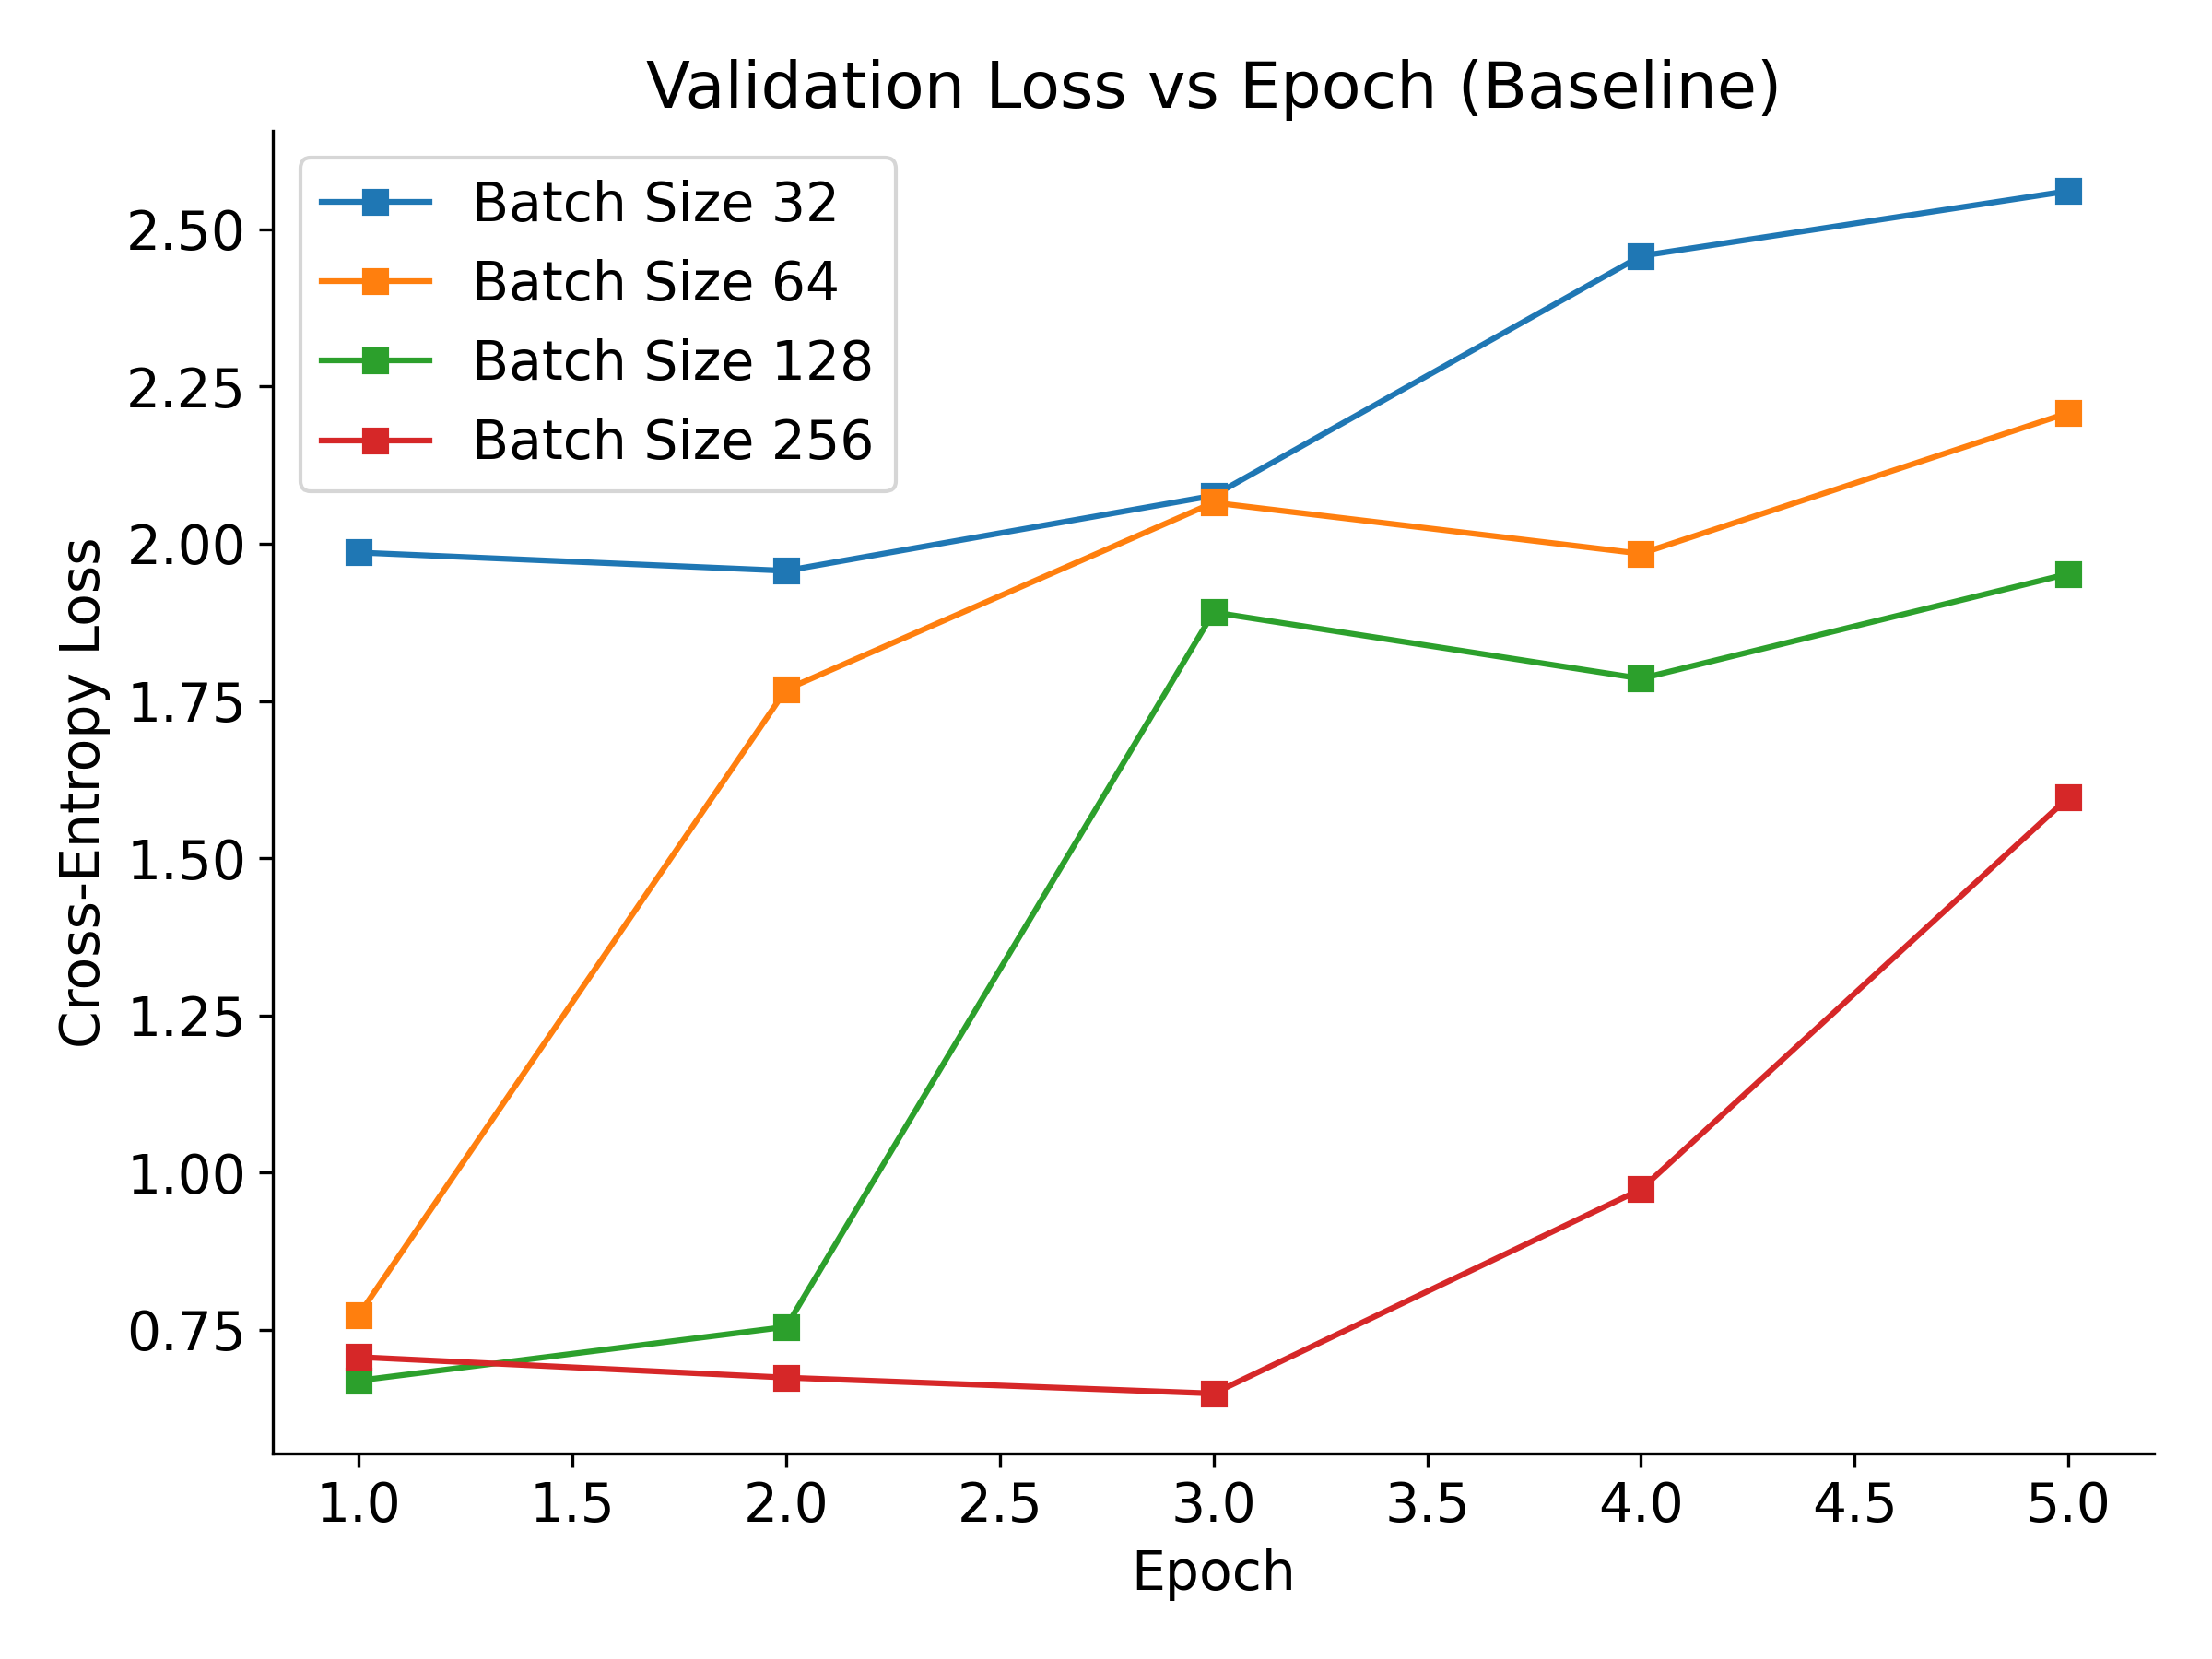
\includegraphics[width=\linewidth]{baseline_val_loss.png}
        \caption{Validation loss over epochs for varying K.}
    \end{subfigure}
    \hfill
    \begin{subfigure}{0.48\linewidth}
        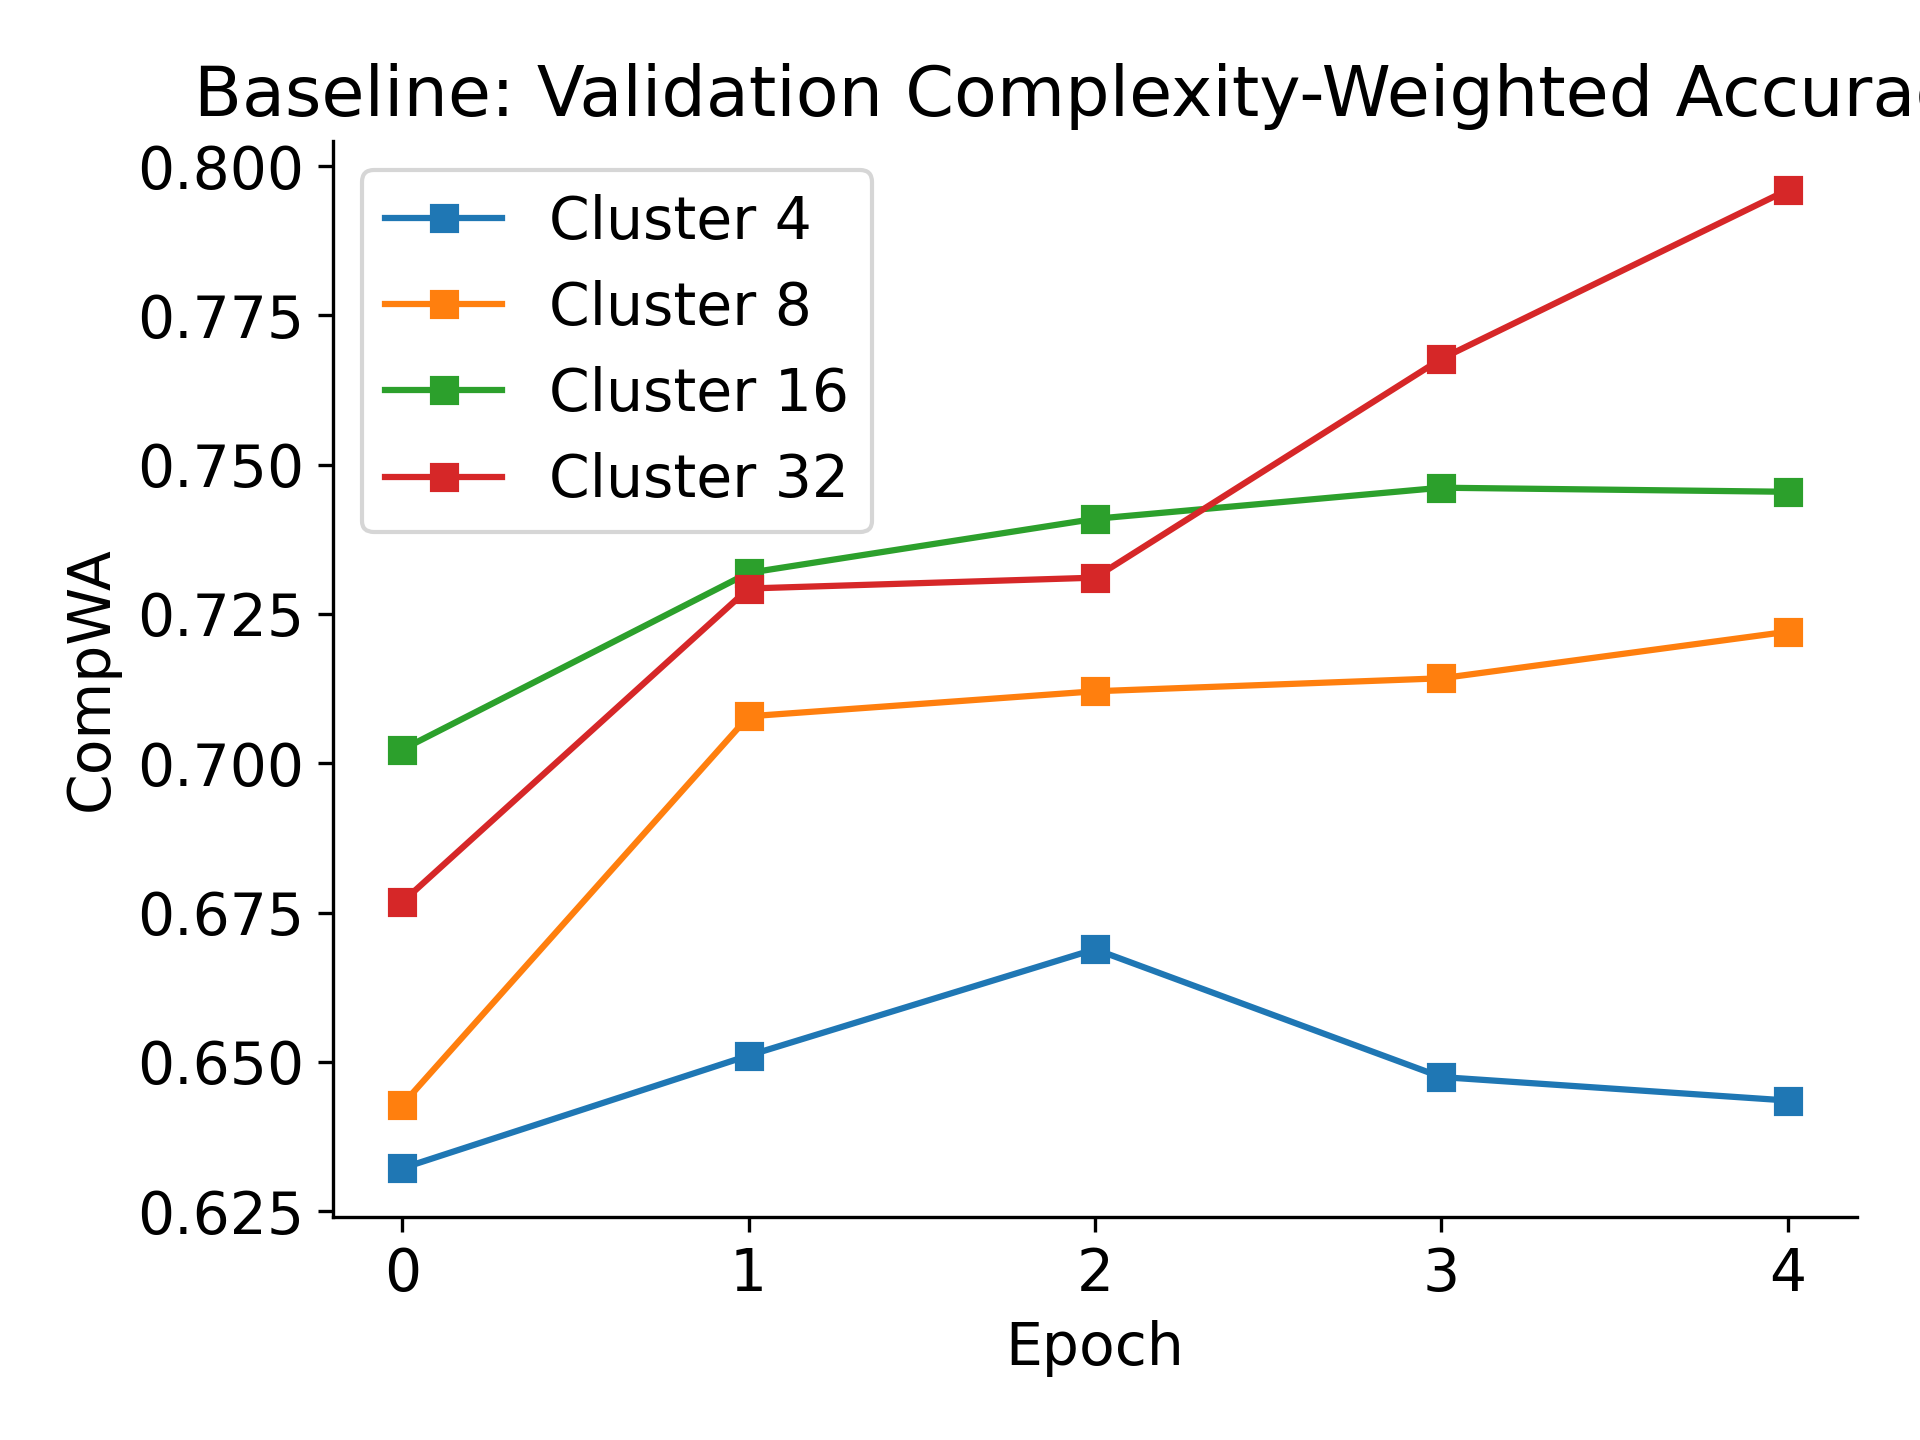
\includegraphics[width=\linewidth]{baseline_val_compwa.png}
        \caption{Complexity-weighted metric for baseline.}
    \end{subfigure}
    \vspace{-1em}
    \caption{Performance metrics for the baseline approach. Higher K-values improve factor granularity but can destabilize training.}
    \label{fig:baseline}
\end{figure}

\begin{figure}[t]
    \centering
    \begin{subfigure}{0.48\linewidth}
        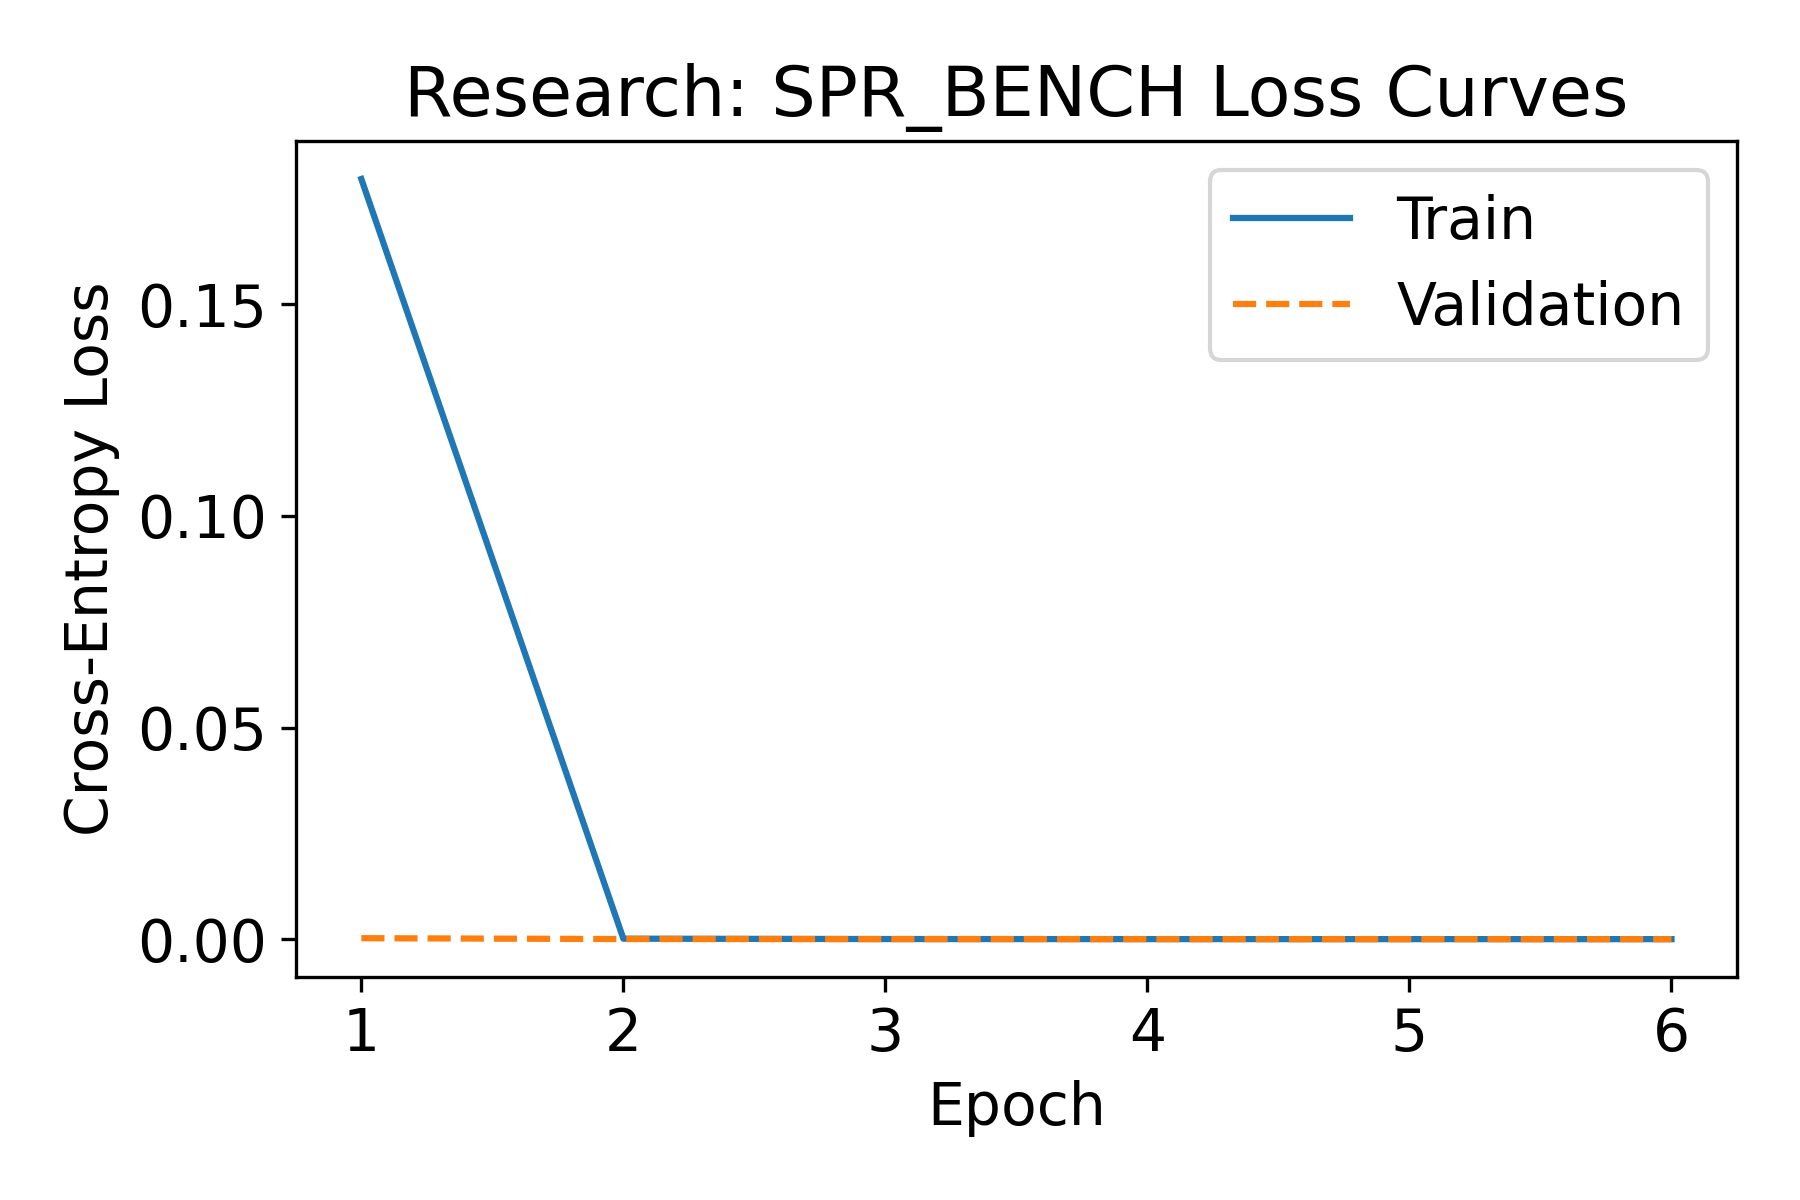
\includegraphics[width=\linewidth]{research_loss_curves.png}
        \caption{Research model loss curves.}
    \end{subfigure}
    \hfill
    \begin{subfigure}{0.48\linewidth}
        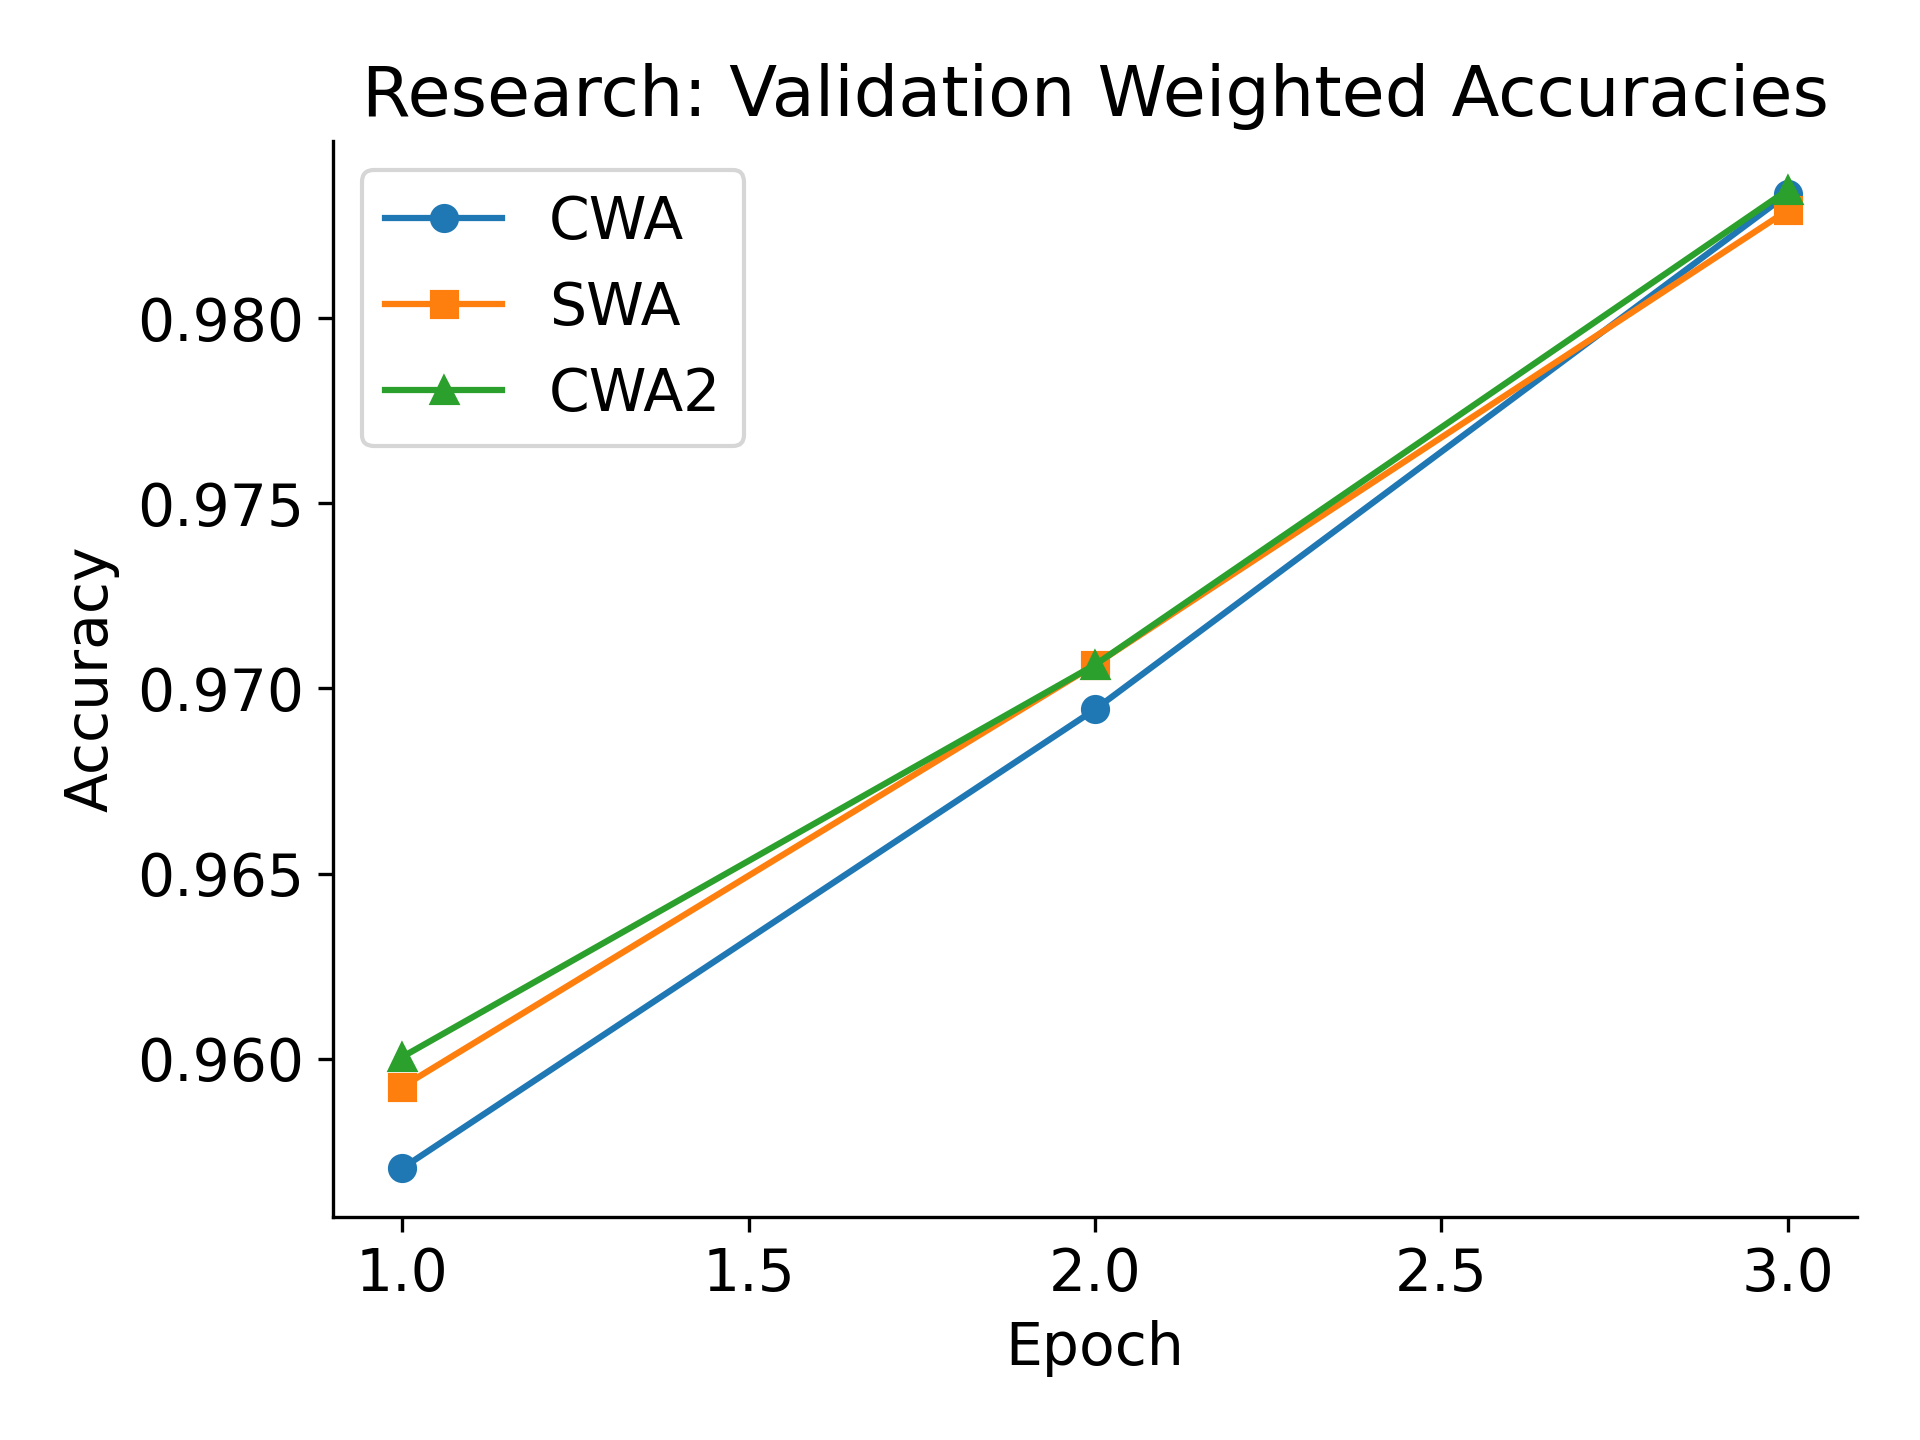
\includegraphics[width=\linewidth]{research_weighted_accuracies.png}
        \caption{Research model weighted accuracy.}
    \end{subfigure}
    \vspace{-1em}
    \caption{In the proposed method, higher complexity weighting leads to more stable performance, yet some trials produce anomalous logs.}
    \label{fig:research}
\end{figure}

The results suggest that data preprocessing and logging protocols must be carefully monitored. Even small interruptions or poorly tuned hyperparameters can derail the learning process. Our partial successes include a sharper performance increase when combining shape and color labels, though the method remains sensitive to initialization.

\section{Conclusion}
We uncovered concrete problems that arise in deep clustering for symbolic tasks, including anomalous training logs and inconsistent performance across seeds. We encourage other researchers to test similar conditions in their pipelines and remain alert to potential pitfalls in K-based factorization. Future work includes refining pipeline components, improving logging resilience, and better uncertainty quantification.

{\small
\bibliographystyle{plainnat}
\bibliography{references}
}

\appendix
\section{Supplementary Material}
Here, we provide additional figures, per-seed lines, and tables to expand on the primary findings. Extended experiments further highlight the fragility of clustering methods under varied hyperparameters and partial label noise. Robust logging infrastructure is critical for reproducible deep clustering research.

\begin{filecontents}{references.bib}
@article{chen2020deep,
  title={Deep clustering: A tutorial},
  author={Chen, Minhao and Li, Tiansheng and Others},
  journal={ArXiv},
  year={2020}
}

@inproceedings{gulrajani2021,
  title={In Search of Lost Domain Generalization},
  author={Gulrajani, Ishaan and Lopez-Paz, David},
  booktitle={ICLR},
  year={2021}
}

@inproceedings{jin2018deep,
  title={Deep Convolutional Clustering and Uncertainty in Disentangled Representations},
  author={Jin, Xu and Logan, Ryan},
  booktitle={NIPS Workshop},
  year={2018}
}

@article{rezende2014stochastic,
  title={Stochastic Backpropagation and Approximate Inference in Deep Generative Models},
  author={Rezende, Danilo J and Mohamed, Shakir and Wierstra, Daan},
  journal={ICML},
  year={2014}
}

@inproceedings{burgess2019monet,
  title={MONet: Unsupervised Scene Decomposition and Representation},
  author={Burgess, Christopher P and Veitch, Matthew and others},
  booktitle={NeurIPS},
  year={2019}
}

@inproceedings{locatello2019challenging,
  title={Challenging Common Assumptions in the Unsupervised Learning of Disentangled Representations},
  author={Locatello, Francesco and Bauer, Stefan and Lucic, Mario and Gelly, Sylvain and Sch\"olkopf, Bernhard and Bachem, Olivier},
  booktitle={ICML},
  year={2019}
}

@inproceedings{wu2020unsupervised,
  title={Unsupervised Shape-Color Disentangling via Clustering},
  author={Wu, Shan and Zhao, Wei and others},
  booktitle={ECCV},
  year={2020}
}
\end{filecontents}

\end{document}